\chapter{Introducción}
\label{cap:introduccion}

\chapterquote{La inteligencia es la habilidad de adaptarse a los cambios}{Stephen Hawking}

%\begin{resumen} En este capítulo se explicará la motivación de este trabajo (Sección %\ref{cap1:sec:Motivacion}), los objetivos que se quieren lograr (Sección %\ref{cap1:sec:Objetivos}) y la estructura de esta memoria (Sección \ref{cap1:sec:Estructura}). 
%\end{resumen}

\section{Motivación}
\label{cap1:sec:Motivacion}

Los seres humanos siempre hemos tenido la necesidad inherente de comunicarnos. La población con dificultades en el lenguaje oral no debe quedar excluida de este derecho, como es el caso de las personas con trastornos del espectro autista, parálisis cerebral, esclerosis múltiple o parkinson, entre otros. 

Para facilitar la comunicación de estos colectivos, se utilizan medios de comunicación
alternativos al lenguaje oral como es el caso de los sistemas pictográficos.
La  manera más común de utilizar este sistema es mediante tableros de comunicación. Estos tableros son superficies  compuestas por una selección de pictogramas, los cuales son imágenes o símbolos que representan una idea o concepto y que permiten al usuario con dificultades de comunicación formar mensajes. Un ejemplo de tablero es el que vemos en la Figura  \ref{fig:tablerofisico}  con el cual el usuario puede señalar un pictograma con el dedo para indicar un objeto u acción. Aparte de los tableros, los pictogramas pueden ser utilizados de otras muchas maneras, como calendarios, agendas, listas de normas, etc.



% TODO: \usepackage{graphicx} required
\begin{figure}[h!]
	\centering
	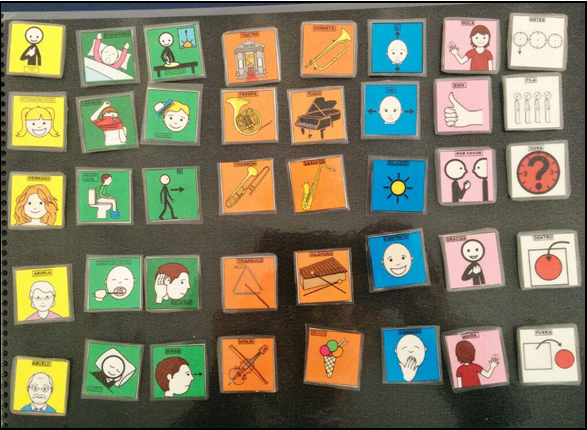
\includegraphics[width=0.7\linewidth]{Imagenes/Bitmap/tablerofisico}
	\caption{Tablero pictográfico en el que el usuario señala lo que quiere comunicar.}
	\label{fig:tablerofisico}
\end{figure}


Los tableros de comunicación a menudo son creados por profesores, padres o tutores para que sean utilizados por una persona con dificultades en el lenguaje. Tradicionalmente se hacían recortando y pegando los pictogramas sobre una cartulina, pero con el tiempo se implementaron soluciones tecnológicas enfocadas a facilitar esta tarea. 

Existen multitud de aplicaciones que permiten crear material basado en pictogramas, pero generalmente están limitadas a un formato concreto y ofrecen poca libertad al usuario para crear material. Además cada una de estas aplicaciones cuentan con opciones y facilidades diferentes, como traducir una frase a pictogramas, un tablero donde se puedan colocar los pictogramas donde se desee, añadir figuras al tablero, etc. Pero no existe ninguna aplicación que englobe todas estas opciones. 

Es por ello que la finalidad de este trabajo es la de crear una aplicación web que permita crear material pictográfico de manera rápida y sencilla, ofreciendo la mayor libertad posible al usuario, e integrando las opciones más utilizadas y demandadas por los usuarios en una única herramienta. 
 





\section{Objetivos}
\label{cap1:sec:Objetivos}



El objetivo del trabajo es desarrollar una aplicación web que permita crear material pictográfico reuniendo las funcionalidades más utilizadas y demandadas por los usuarios. La aplicación debe contar con un tablero que permita desplazar los pictogramas y otros elementos complementarios con precisión.

Para ello, se investigarán las distintas aplicaciones existentes y cuáles son las funcionalidades más reclamadas por los usuarios. También se investigarán y ampliarán conocimientos sobre distintas tecnologías web actuales. 

Otro objetivo es la de crear una interfaz sencilla e intuitiva para el usuario que pueda ser utilizada en el mayor número de dispositivos posible. Para contrastar los objetivos del trabajo, se realizará una evaluación donde se compruebe la facilidad de uso de la aplicación. 










\section{Estructura de la memoria}
\label{cap1:sec:Estructura}

La estructura para memoria se encuentra dividida en ocho capítulos cuyo contenido se explicará brevemente a continuación: 
\begin{itemize}
	\item En el capítulos uno, en español y en inglés expondrá el contexto bajo el cual se ha realizado el trabajo junto a la motivación y objetivos para realizarlo.
	
	\item En el capítulo dos se explicará qué es un pictograma y los distintos sistemas de comunicación basados en ellos. Además se analizarán las distintas herramientas relacionadas con pictogramas haciendo énfasis en la edición de tableros.
	
	\item En el capítulo cuatro se presentarán las tecnologías utilizadas para el desarrollo de la aplicación.
	
	\item En el capítulo cuatro se especificarán los requisitos y explicarán los prototipos creados.
	
	\item En el capítulo cinco se explicará en detalle la arquitectura e implementación de la aplicación.
	
	\item El capítulo seis mostrará el diseño, resultado y análisis de la evaluación realizada por los usuarios. 
	
	\item En el capítulo siete, en español y en inglés se presentarán las conclusiones finales y se especificará el trabajo futuro a realizar.
	
	\item En el capítulo ocho se detallarán las tareas realizadas por los dos integrantes del proyecto.
\end{itemize}	




